\documentclass[11pt, letterpaper]{article}
\usepackage{graphicx}
\usepackage[export]{adjustbox}
\usepackage{hyperref}
\usepackage{xcolor}
\graphicspath{{images/}}
\usepackage[a4paper, total={6in, 8in}]{geometry}
\usepackage{tabularx}
\usepackage{float}


\title{\textbf {Audio classification with machine learning} \\ \large Introduction to Machine Learning 2024/2025Z}

\author{Łukasz Górski \\ Piotr Iśtok \\ Piotr Jacak \\ Stanisław Janowicz \\ Marcin Falkowski}

\date{Styczeń 2025}


\begin{document}
\maketitle

\newpage
\tableofcontents
\newpage

\section{Abstract}

The task we will be attempting to solve in this project is a binary recognition problem, meaning that the program's main function is to transform a given input into either 1 or 0, depending on certain properties and conditions. Specifically, the input will consist of a single audio file, either uploaded directly or recorded on a recorder with a microphone by the program. We will transform this audio file into a spectrogram and, after cleaning and pre-processing, pass it into the model to determine its membership in class one, representing the people who are granted access, or class zero, or the people who are denied.

The intended use of this project is on a voice-based intercom device that must discern whether a person has the authority to enter restricted areas.

\section{Introduction}

In this section we present some useful background information on audio classification and on the more technical aspects of the project.

\subsection{Audio Classification}
 Audio classification is a machine learning task that involves identifying and tagging audio signals into different classes or categories. In our case, this is done through the analysis of spectrograms of the files provided, since analysis of images is used much more frequently in the field of machine learning.

 Our data set is the \href{https://www.kaggle.com/datasets/psyreddy07/daps-data}{DAPS} set, consisting of .wav files of 20 speakers reading 5 scripts each, averaging at about 14 and a half minutes.

 Of those 20 speakers, F1, F7, F8, M3, M6, M8, are chosen as class 1, and the other speakers form class 0.

 \subsection{Convolutional Neural Networks}
 The model used is a Convolutional Neural Network (CNN), which is a common type of deep learning network employed in tasks of recognition, especially image processing. It consists of an input layer, a number of hidden layers, and an output layer. In our program, the output layer is binary, since we only have 2 classes.

 We chose the \verb|pytorch| library to implement our model.

\section{Cleaning and pre-processing}

\subsection{Preprocessing}
Effective preprocessing of audio data is a critical step in achieving high-quality features for machine learning models. In this project, preprocessing ensures uniformity across audio samples and eliminates irrelevant segments.
\subsubsection{Sample Rate}
In speech-related tasks, consistency in the sample rate is vital to ensure that all audio files have the same temporal resolution. We decided to set the base sample rate to 16kHz (Wideband frequency), because it is used in most modern VoIP (Voice over Internet Protocol) and is a extension over standard 8kHz narrowband. For us it was perfect balance between computational efficiency and retaining the critical sampling frequency.
\subsubsection{Removing Silent Parts}
Silence in audio fragments often contains no meaningful information for speaker recognition and can introduce noise or inflate the data size unnecessarily. To address this, silent parts of the audio were detected and removed during preprocessing. This step ensures that the input to the model focuses solely on speech, improving training efficiency and performance.

\subsection{Cleaning}
In machine learning applications that involve audio data, such as speaker identification, the quality of the input signal is critical. Background noise can obscure important voice features, which can lead to reduced model performance. One way of overcoming this issue and improving SNR (signal to noise ratio) is denoising data using spectral gating. It works by computing a spectrogram of a signal (and optionally a noise signal) and estimating a noise threshold (or gate) for each frequency band of that signal/noise.
That threshold is used to compute a mask, which gates noise below the frequency-varying threshold. The main reasons why it is a good option for reducing noise are:
\begin{itemize}
    \item \textbf{Preservation of signal features:}
        Spectral gating works in the frequency domain, selectively weakening noise-dominated frequencies, keeping the structure of our target signal (voice) mostly intact.
    \item \textbf{Flexibility:}
        The method uses a noise profile derived from a sample with only background noise, which allows our program to adapt to different environments such as street noise, electrical noise and reverberation. Because of it our code is simple without any noticeable performance drop.
    \item \textbf{Ease of use:}
        This method of denoising is implemented in the free-to-use Python library called "noisereduce", keeping our solution easily reproducible and can be seamlessly integrated into our pipeline.
\end{itemize}
Unfortunately, spectral gating also has its drawbacks. The biggest one is that, for it to work there needs to be a noise sample provided, which can be for us sometimes impossible to distinguish. That's why in that case our denoising step in pipeline will use band-stop filter, implemented with Butterworth filter. The main advantages of it are:
\begin{itemize}
    \item \textbf{No need for a noisy sample:}
        This filter always removes lower frequencies, so urban sounds can be easily eliminated, without the need of noisy sample.
    \item \textbf{Preservation of higher frequencies:}
        The Butterworth filter's characteristic smooth frequency response ensures minimal distortion in the preserved higher frequencies.
    \item \textbf{Preprocessing Simplicity:}
        This approach is computationally efficient and easy to implement.
\end{itemize}
The reason why it is not used all the time is that it has many limitations. It is not ideal for broadband noise. It may not effectively remove all of it. The other one is that it overlaps with voice frequencies, so it can also attenuate it resulting in reduced intelligibility.\\We also considered using deep learning for audio cleaning, as it has shown great potential by leveraging neural networks to learn complex mappings between noisy and clean audio signals. However, we came to the conclusion that it is too advanced a tool to remove such simple noises and two methods described before are efficient enough.

\subsection{Spectrograms}
In speaker recognition tasks, the selection of an appropriate feature extraction method is crucial. The acoustic properties of human speech vary widely and capturing these nuances effectively is essential for accurate classification. Among many methods for converting raw audio signals into a form suitable for machine learning, it was imposed on us to use spectrograms. We created three types, however in the final version only one of three listed down below methods is used.
\begin{itemize}
    \item \textbf{Regular Spectrogram}
        This method computes the spectrogram by applying the Short-Time Fourier Transform (Stft) to the audio signal. It visualizes how the signal's frequency content varies over time. While this approach provides an accurate representation of raw frequency components, it does not consider the perceptual differences in how humans interpret sound.
    \item \textbf{Spectrogram with adjustable parameters and dB scale}
        This method allowed us to changed parameters such as FTT size, window size and hop size. However tweaking those parameters didn't bring any improvements. The biggest advantage of this method compare to the previous one is dB scaling of spectrogram. Because of that more features were clearly shown.
    \item \textbf{Mel Spectrogram}
        The mel spectrogram method transforms the audio signal into a representation that closely matches the human ear's sensitivity to frequency. It maps the frequencies to the mel scale, which emphasizes lower frequencies (important for speech) while de-emphasizing higher, less perceptible frequencies. By focusing on perceptually relevant features, the mel spectrogram strikes a balance between simplicity, efficiency, and effectiveness. It directly produces features well-suited for downstream models without requiring extensive manual adjustments. To no surprise, this method we had the best results so it is being used in final version.
\end{itemize}
Additionally all spectrograms are stored in grayscale to take up as little space as possible without loosing important data for further usage.

\section{Exploratory Data Analysis}

Exploratory Data Analysis (or EDA for short) is the process of gathering information from the given data set before using it for the purposes of informed decision making later on. Since our data are in the form of .wav files, we use the \verb | scipy.io.wavfile |Python library to load it in order to analyze it by looking directly at the array representing it. This was our first attempt at EDA, and although the code itself runs quick, it gives us very little useful information. Namely, we only have access to the numbers: the minimum and maximum values of the array, the means, sample rates and the lengths of the files in each class. This is hardly enough - the length of an audio doesn't, and shouldn't, affect how is it classified.

Therefore, we make use of Python libraries that are more suited to accomplishing our goals. After presenting the audio in the form of spectrograms, we extract helpful details into a .csv file, which becomes the input of the next stages of EDA. The details shown in the .csv vary greatly from the simple values of the previous step and are of much greater importance to us. Here are the features that we managed to extract in this way: Person, sex, script, audio type, is a test set, class, and contrast. Let us explain them one by one:
\begin{itemize}
    \item Person - the person speaking in the audio, as described in the Data section,
    \item Gender - the gender of the person (either male or female),
    \item Script - the script read in the audio,
    \item Audio Type - type of audio (either cleanraw, ipadflat, ipad, or iphone)
    \item Is Test Set - a binary value describing whether the file was used in training the model or testing it,
    \item Class - 0 or 1, as described in the Introduction
    \item Contrast - the contrast of the image.
\end{itemize}
Besides these values, there were five other features - average RGB values of the image as well as the Brightness and Saturation. However, as discussed in the Spectrograms section, the spectrograms were in grayscale, making all of these values equal to each other, and thus redundant. Because of this, we have decided to analyze only the mean redness value of the images with the understanding that it also signifies the other features from this section.

With this data, we can begin presenting the previously-numerical information visually, which makes the insights much more obvious to a human observer. We make use of the \verb|seaborn| library to generate histograms like the following:

\begin{figure}[H]
    \centering
    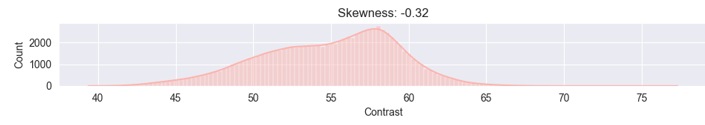
\includegraphics[width=1\linewidth]{image.png}
    \caption{Contrast distribution}
    \label{fig:enter-label}
\end{figure}

We can than utilize the same library to plot pairwise relationships in the data set, checking to what degree two variables are correlated with each other. Using the \verb|heatmap| function, we get the following result:

\begin{figure}[H]
    \centering
    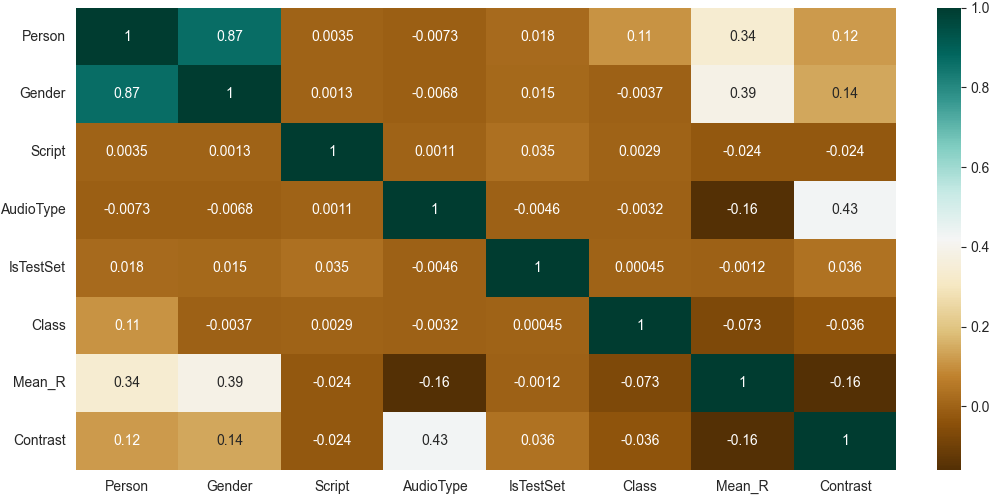
\includegraphics[width=1\linewidth]{pairplot.png}
    \caption{Pairwise relationships in the data set}
    \label{fig:enter-label}
\end{figure}

Lower values indicate a negative correlation between two variables, while values closer to 1 mean a positive association. From this heatmap, we can conclude that the Gender and Person variables are correlated, which means that the data set isn't split evenly between male and female recordings. This is a valuable insight, since it might affect model - if we chose the training set from the original data at random, the model might be worse at classifying one gender than the other.

Fortunately, looking at the value of the intersection between Gender and IsTestSet (0.015), the test set itself is fairly balanced.

To better understand our data we decided to explore the impact of different kinds of spectrograms on tested values. Thanks to this we could try and predict which method of creating spectrograms could improve our model. This way we could skip testing model for every method of generating spectrograms, since the process is very time-consuming. Predictions were based on comparing features of spectrograms which gave good results to those with bad ones. 

First, however, we had to choose the training set and the testing one. We decided that it was vital that the distribution of data in each set is similar, and we made sure that no fragment of audio is used in both sets.  The results of our tests were satisfactory, and we proved that the proportions of main features such as audio type, speaker, gender or the script being recited, are similar for both sets.

At this point, it is worth noting that even though distribution of audio in the whole dataset based on gender was similar, the amount of audio provided by individual speakers could vary greatly (which could negatively impact the recognition of some speakers compared to others). Other features resulting from spectrograms were also similar for each set (with the method for creating spectrograms we choose in the end giving the best results). 

We noticed that every speaker had very noticeable traits which were reflected in the features we got from inspecting spectrograms, some methods gave slightly better results than others. There is no such distinction between groups labeled for entry and others, however. It is assumed that no matter which method of creation was used, this situation would not change, as the number of speakers in each class is random (not related in means other than class).

Different kinds of spectrogram models gave different results in terms of compared features. In the end the best results were given by MEL-type spectrograms. Those spectrograms were superior in reflecting differences between different speakers and their genders, while having similar effects no matter for which audio tape they were used on. The CNN model using them had best results compared to other types of spectrograms.

\section{Model Training}
\subsection{Dataset}

The dataset used for this project consists of voice samples cut into 2-second fragments. To guarantee that all the fragments of a voice sample end up in the same set, we decided to choose recordings randomly and assign them to either the training set or the test set as follows:

\begin{itemize}
    \item \textbf{Training set}: 85\% of the data, which is 1100 out of 1300 recordings.
    \item \textbf{Test set}: 15\% of the data, which is 200 out of 1300 recordings (60 from class 1 and 140 from class 0 to keep proportions even).
\end{itemize}

\subsection{Model Testing}

Testing various models started with a simple network from the PyTorch tutorial. We used the simplest spectrograms for this one, with a linear scale. The purpose of this model was to get a grasp of how everything works and ensure we could proceed with more advanced models. Since the images were quite large for machine learning, we resized them to ¼ of their size in each dimension. This gave us a macro-averaged F1-score of 0.72 (on the test set).

Shortly after, we tested a very similar model, with the main change being the addition of more epochs (from 3 to 10), which naturally improved the result to an F1 score of 0.78, which was satisfactory for the first stage.

\subsection{Second Stage: Advanced Model}

During the second stage, we decided on a slightly more advanced model with 3 convolutional layers and 2 fully connected layers. We kept using the SGD optimizer, 10 epochs, and a batch size of 64 as in the first stage. We did not want to overcomplicate this model, as the main purpose was to decide which spectrograms were the best. Data analysis suggested that some of them could be better, but theory only takes you so far, so we decided to train a model using the same network for each type of spectrogram:

\begin{enumerate}
    \item First, we tried mel spectrograms, which we believed to be the best. With an F1 score of 0.9, it was a noticeable improvement over the previous stage, but not the best yet.
    \item The second type of spectrograms we tested were spectrograms with a logarithmic scale. They appeared to be better than the mel ones, as the model gave us an F1 score of 0.94.
    \item To ensure completeness, we tried the first type again (linear scale), and the result was the worst, with an F1 score of 0.85.
    \item To improve the spectrograms (especially the mel ones), we changed the sampling rate to 16000. In the case of spectrograms 2, it increased the F1 score to 0.95.
    \item The improvement was more noticeable for mel spectrograms, allowing us to achieve an F1 score of 0.955.
    \item We tried noise removal as well. However, the results were not the best, as the F1 score dropped to 0.94 for mel spectrograms. While it is not a significant drop, we decided not to use this idea in the next stages. Although the audio sounded better to the human ear after noise removal, it clearly was not better for machine learning. Most likely, it removed some features from the recording that were not noticeable to us but were useful for the training process.
    \item Similarly, spectrograms 2 also got worse after removing the noise, as the F1 score dropped to 0.93, further proving that noise removal did not work as intended.
    \item We attempted audio normalization (using the librosa.pcen function) on our 16000 mel spectrograms, but it also made them worse, giving an F1 score of 0.93.
\end{enumerate}

As a result of these experiments, we decided to use mel spectrograms with a 16000 sampling rate to train the next models, as they appeared to be the most accurate. Alternatively, we could try using spectrograms 2. We did not create the 16000 sampling rate or noise removal versions of the linear spectrograms, as they were clearly the worst and could not possibly outperform the others.

\subsection{Further Tests}

During further tests, we tried changing the transform to resize the images to only ½ of their original size in each dimension. While it seemed promising at first, as the loss started decreasing very rapidly (as seen in the figure), the result was comparable to that of the previous model, with an F1 score of 0.94.

\begin{figure}[H]
    \centering
    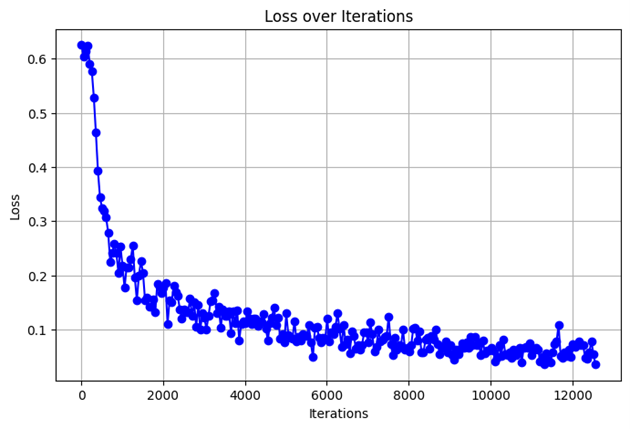
\includegraphics[width=0.8\textwidth]{lossplot1.png}
    \caption{A graph showing the change in loss values during training}
\end{figure}

Another model was an attempt at something more experimental, as we tried a different activation function (LeakyReLU instead of ReLU) and added batch normalization. However, as a result of unnecessary additions (most likely adaptive average pooling, which was not needed here), the model ended up being greatly overfitted, with an F1 score of 0.77 on the test set compared to 0.94 on the training set.

\subsection{Most Successful Model}

Our most successful model was similar to the one we tested all our spectrograms on, but with the addition of batch normalization and an additional fully connected layer, giving us 3 convolutional layers and 3 fully connected layers. On top of that, we changed the optimizer to Adam. The results were by far the most satisfying, as we got an F1 score of 0.966 after only 10 epochs. Batch normalization seemed to be key in this case.

Since it was our most accurate model, we decided to experiment further and test how much the number of epochs would affect the result. After 30 epochs, the accuracy improved only slightly (0.968 F1), which was not as much as we expected. After another 30 epochs (giving a total of 60), the results did not improve at all. All of this can be noticed in the figure showing the change in loss values during training. Halfway through the training process, we reached a plateau, and the model stopped learning. We also tried a different approach, in which we changed the learning rate throughout the training to a lower value (from 0.001 to 0.0002), but it also did not help much, giving more or less the same accuracy for both sets.

\begin{figure}[H]
    \centering
    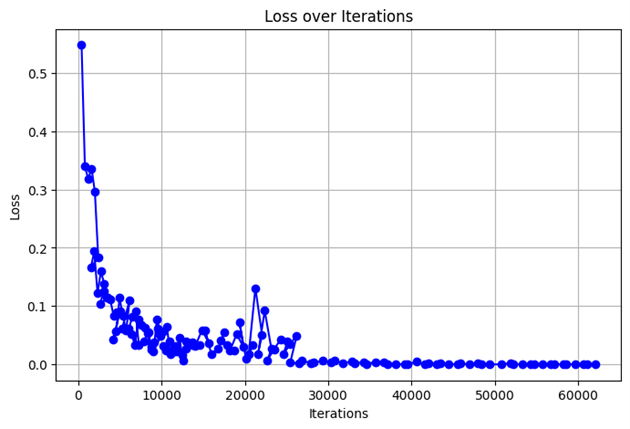
\includegraphics[width=0.8\textwidth]{lossplot2.png}
    \caption{A graph showing the change in loss values during training of our best model}
\end{figure}

\subsection{Final Attempts}

Next, we attempted to improve our model by increasing the number of layers (4 convolutional, 3 fully connected), changing the dropout probability, changing the parameters of the layers, and changing the batch size (from 64 to 32 or 128), but none of these proved effective. All these models hovered around an F1 score of 0.95, making them slightly worse than our best one.

During our last attempts, we tried changing our spectrograms a bit by resizing them differently, as many sources on the internet used images of size 64x64. However, this also did not achieve anything interesting, as the result was comparable to previous ones.

\section{Conclusion}

In conclusion, it seems that we hit a kind of barrier around 0.96-0.97 f1, and without some major changes to the way we create our model or some solid data augmentation, getting our model to reach an F1 score of 0.98 or higher seemed improbable.

\end{document}
